\documentclass[twocolumn]{article}
\usepackage{graphicx}
\usepackage[utf8]{inputenc}
\usepackage[a4paper, margin=0.79in]{geometry}
\usepackage{lastpage}
\usepackage[compact]{titlesec}
\usepackage{tikz}
\usepackage{float}
\usepackage{listings}
\usepackage{multicol}
\usepackage{graphicx}
\usepackage{hyperref}
\usetikzlibrary{fit}

\titleformat{\section}[hang]{\bfseries\large}{\thesection}{0.5em}{}
\titleformat{\subsection}[hang]{\bfseries\normalsize}{\thesubsection}{0.5em}{}
\titleformat{\subsubsection}[runin]{\bfseries\normalsize}{\thesubsubsection}{0.5em}{}



\title{\large{\textbf{Wireless IoT and LAN (CESE4060): Matlab or NS3 Report}}}
\author{
    \small Tobias Veselka (4451848, tobiasveselka1) \and
    \small Enes Kaya (5279003, ekaya)
}
\date{\today}

\begin{document}

\maketitle

\begin{center}
    \footnotesize{Report contains \pageref{LastPage} of maximum 4 pages.}
\end{center}

\section{Idea behind our Approach}

The central question of this investigation is: \emph{under which network conditions does IEEE~802.11ax OFDMA improve system performance compared to 802.11ac-like single-user TDMA scheduling?} In 802.11ax, the access point (AP) can serve multiple stations simultaneously by assigning each to a dedicated Resource Unit (RU) within the same transmission window — a mechanism known as downlink OFDMA. In contrast, 802.11ac schedules users sequentially, dedicating the full channel bandwidth to one user per time slot.

The intuition is that OFDMA should help when users have heterogeneous demands or widely varying channel conditions: instead of wasting air-time on sequential transmissions for users with small payloads or poor channels, the AP can batch all users into a single parallel slot. However, this comes at a cost. The shared OFDMA slot is bounded by the \emph{longest} user frame in the round — what we call the bottleneck-slot effect — meaning users with small packets or low MCS occupy a disproportionately large slot. We designed two scenarios to probe when this trade-off works in favour of OFDMA and when it does not.

\section{Implementation}

Simulations were carried out in MATLAB using the WLAN Toolbox. The 802.11ac baseline used \texttt{wlanVHTConfig} and \texttt{wlanWaveformGenerator} with round-robin TDMA over an 80\,MHz (CBW80) channel. The 802.11ax system used \texttt{wlanHEMUConfig} (allocation index~112, 996-tone RU) so that all users are served within a shared slot of duration $T_\text{slot}^\text{ax} = \max_u T_u^\text{ax}$. Channel propagation was modelled with \texttt{wlanTGaxChannel} (Model-B delay profile, independent fading per user), with AWGN added via \texttt{awgn} at the per-user target SNR. Channel estimation used \texttt{wlanVHTLTFChannelEstimate} (ac) and \texttt{wlanHELTFChannelEstimate} (ax); data recovery used \texttt{wlanVHTDataRecover} and \texttt{wlanHEDataBitRecover}. LDPC channel coding was used throughout, and 50 packets per user were simulated.

Per-user throughput in 802.11ac is $T_u^\text{ac} = B_u \,/\, (N \cdot T_u^\text{ac} \cdot N_\text{usr})$, since each user waits through $N_\text{usr}-1$ other slots. In OFDMA, $T_u^\text{ax} = B_u \,/\, (N \cdot T_\text{slot}^\text{ax})$. Packet delay in 802.11ac includes a queuing component $(u{-}1)\,T_u^\text{ac}$; OFDMA has zero queuing but charges every user the full bottleneck-slot duration. Jain's Fairness Index was computed on per-user throughputs: $\text{JFI} = (\sum x_i)^2 \,/\, (N_\text{usr} \cdot \sum x_i^2)$.

Key assumptions: perfect channel knowledge at the receiver, SISO links only, no closed-loop feedback or MU-MIMO, and large-scale fading disabled to isolate multipath and SNR effects.

\section{Results}

\subsection{Scenario A: Heterogeneous Traffic}

\subsubsection{Setup and Hypothesis.}
Four users were configured with two traffic profiles: two \emph{video} users (1500\,B payload, MCS~8/10 for ac/ax, 30\,dB SNR) and two \emph{voice} users (128\,B, MCS~4/5, 25\,dB SNR), all at close distances (3--9\,m). We hypothesised that in round-robin TDMA, large-payload video users would dominate aggregate throughput due to their high MCS, creating an unfair outcome for voice users. OFDMA was expected to equalise per-user throughputs at the cost of reduced aggregate performance, because the voice users' short frames would force a waste when the bottleneck slot is set by the video users.

\subsubsection{Throughput.}
\autoref{fig:a_total_tp} shows 802.11ac achieving 109.9\,Mbps aggregate versus only 31.3\,Mbps for 802.11ax — roughly $3.5\times$ worse. Per-user throughput (\autoref{fig:a_user_tp}) reveals the cause: video users reach $\approx$40\,Mbps with 802.11ac but only $\approx$7\,Mbps with OFDMA, while voice users achieve $\approx$7--9.5\,Mbps in both systems. The bottleneck-slot effect is responsible: voice payloads are 128\,B, but the shared slot is governed by the 1500\,B video frames, charging voice users a slot far longer than they require to transmit their own data. Video users are similarly penalised — their bandwidth is now shared with voice users rather than dedicated.

\begin{figure}
    \begin{minipage}{0.45\textwidth}
        \centering
        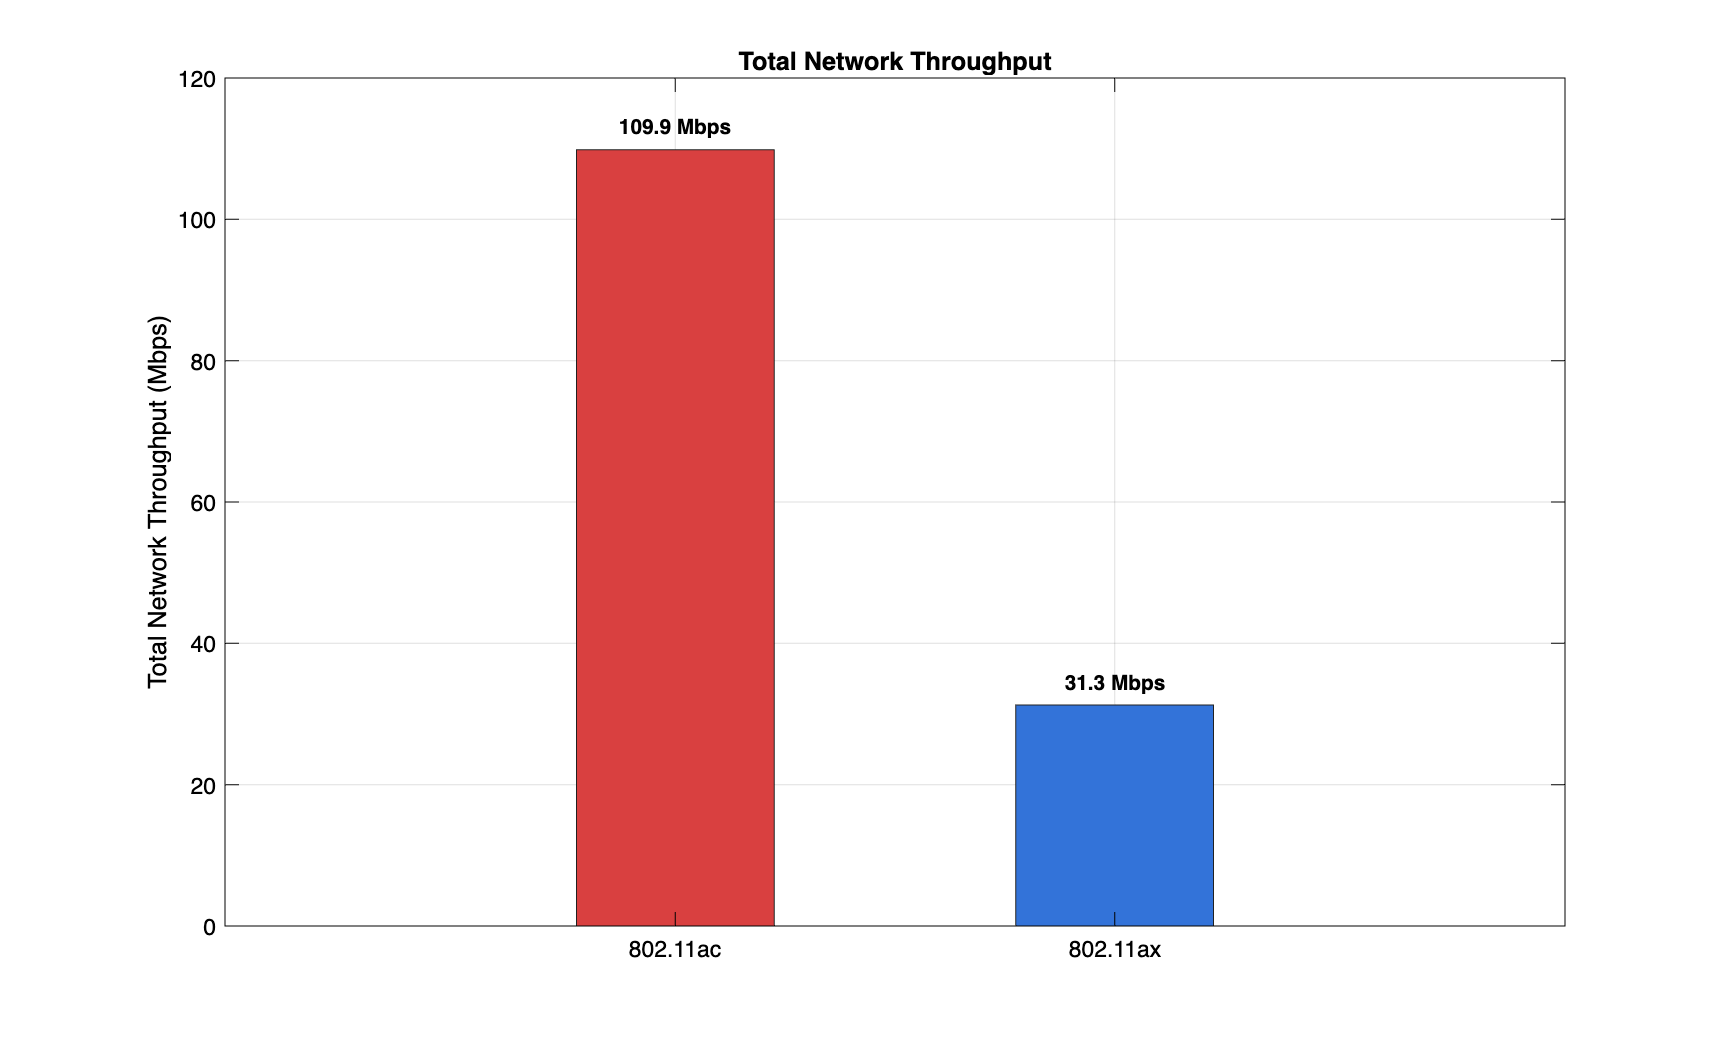
\includegraphics[height=3.9cm]{figures/scenario-a/total_network_throughput.png}
        \caption{Scenario A: Total network throughput. OFDMA performs significantly worse in aggregate.}
        \label{fig:a_total_tp}
    \end{minipage}\hfill
\end{figure}

\begin{figure}
    \begin{minipage}{0.45\textwidth}
        \centering
        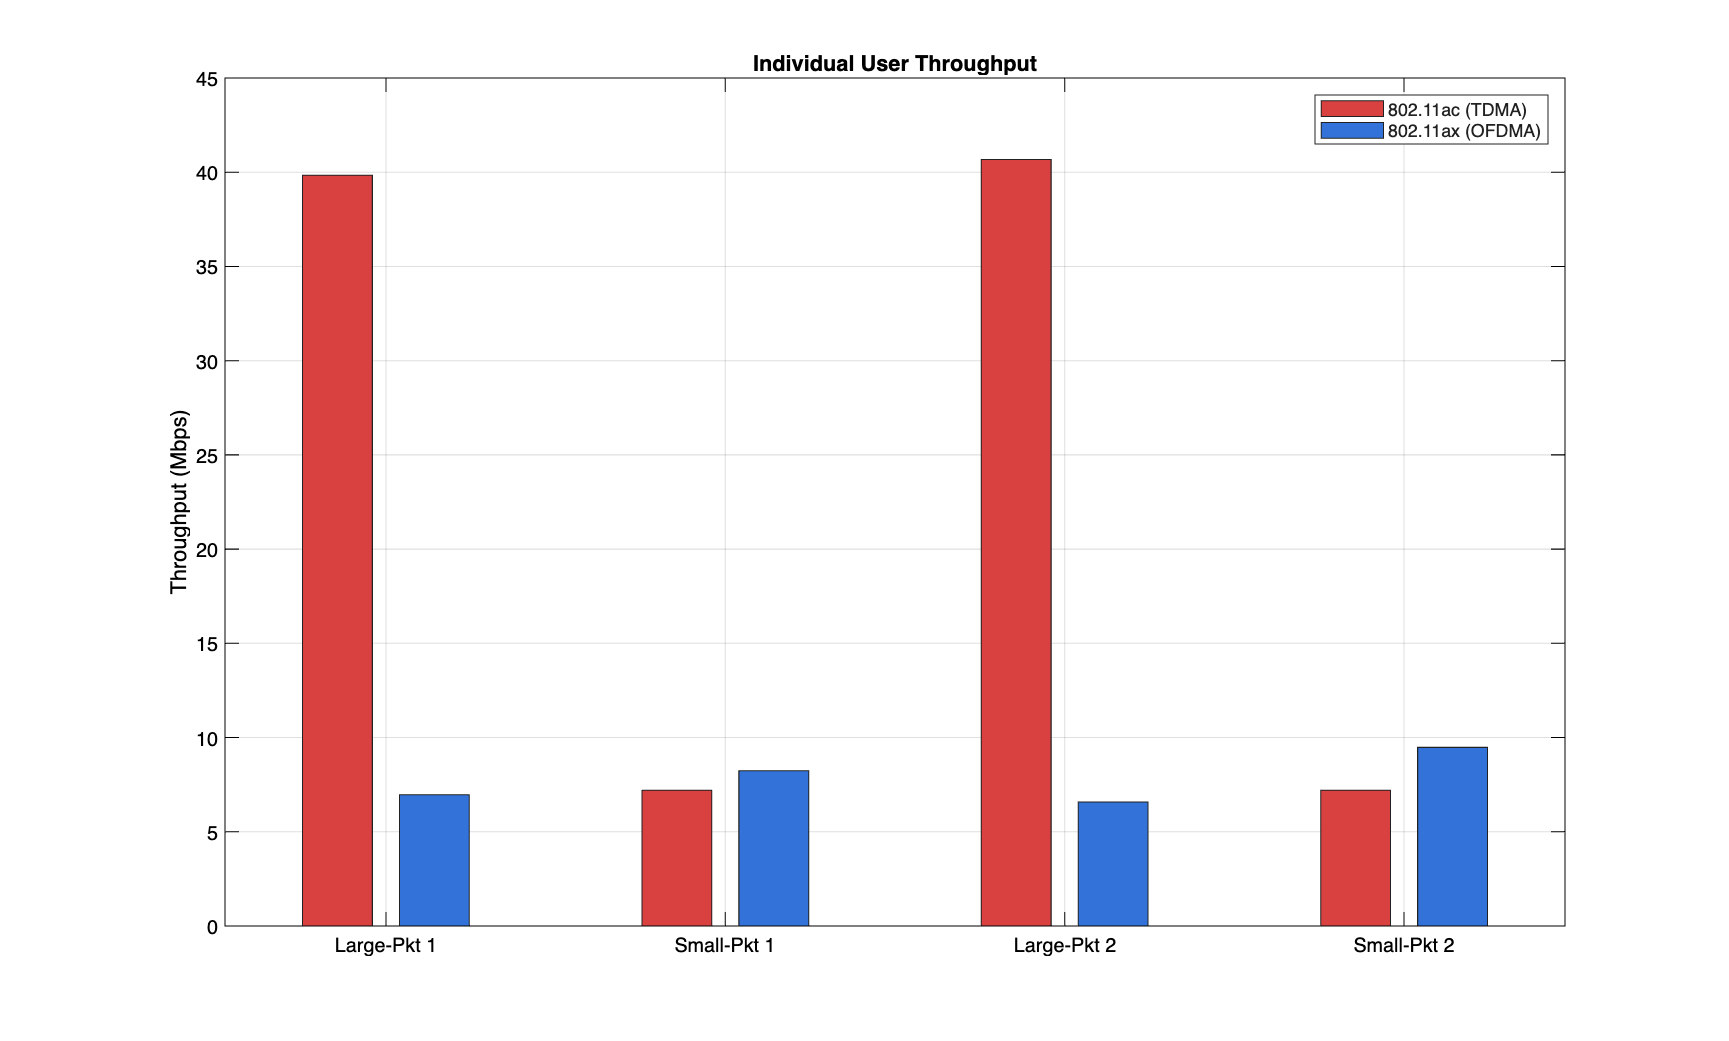
\includegraphics[height=3.9cm]{figures/scenario-a/individual_user_throughput.png}
        \caption{Scenario A: Per-user throughput. OFDMA equalises users while TDMA favours large-packet users.}
        \label{fig:a_user_tp}
    \end{minipage}\hfill
\end{figure}

\subsubsection{Fairness and Spectral Efficiency.}
Jain's Fairness Index (\autoref{fig:a_jfi}) rises from 0.675 (802.11ac) to 0.994 (802.11ax). This confirms our hypothesis: round-robin TDMA strongly advantages high-MCS, large-payload users, while OFDMA's shared slot normalises their throughputs towards near-perfect fairness. The per-user spectral efficiency (\autoref{fig:a_user_se}) adds an important nuance: voice users see their per-user SE jump from $\approx$0.09\,bps/Hz (sharing 80\,MHz in TDMA) to $\approx$0.43\,bps/Hz (with a dedicated 20\,MHz sub-band in OFDMA). This indicates that for small-packet users who would otherwise be allocated a full wide-band slot they cannot efficiently use, OFDMA's sub-band dedication offers a genuine spectral gain at the user level.

\begin{figure}
    \begin{minipage}{0.45\textwidth}
        \centering
        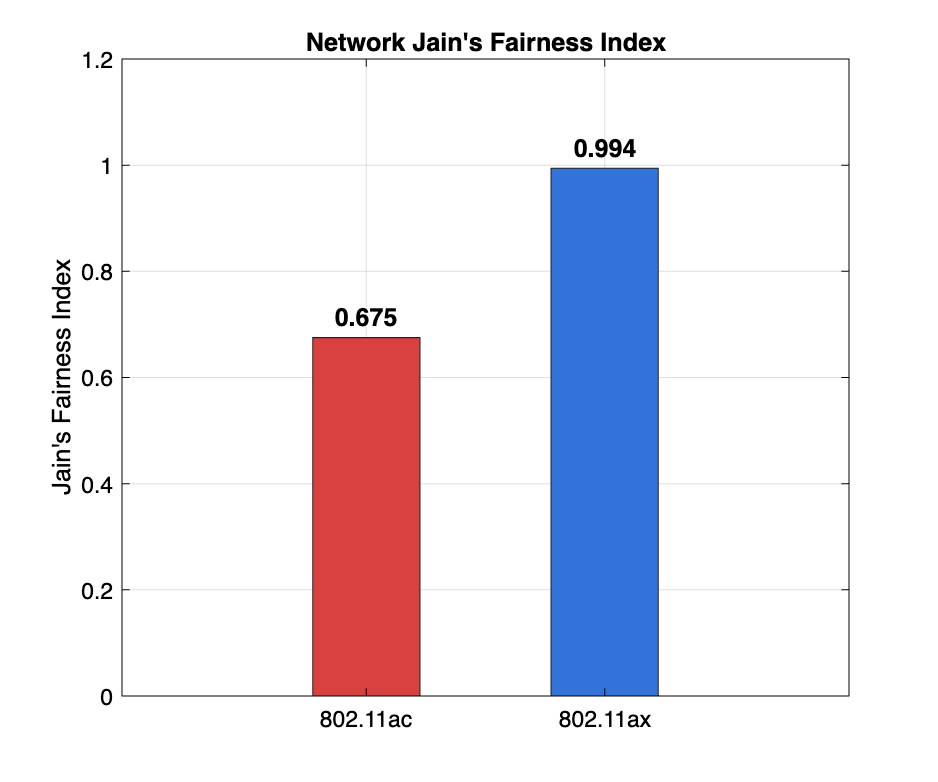
\includegraphics[height=3.9cm]{figures/scenario-a/jain_fairness_index.png}
        \caption{Scenario A: Jain's Fairness Index. OFDMA dramatically improves fairness to near-perfect.}
        \label{fig:a_jfi}
    \end{minipage}\hfill
\end{figure}

\begin{figure}
    \begin{minipage}{0.45\textwidth}
        \centering
        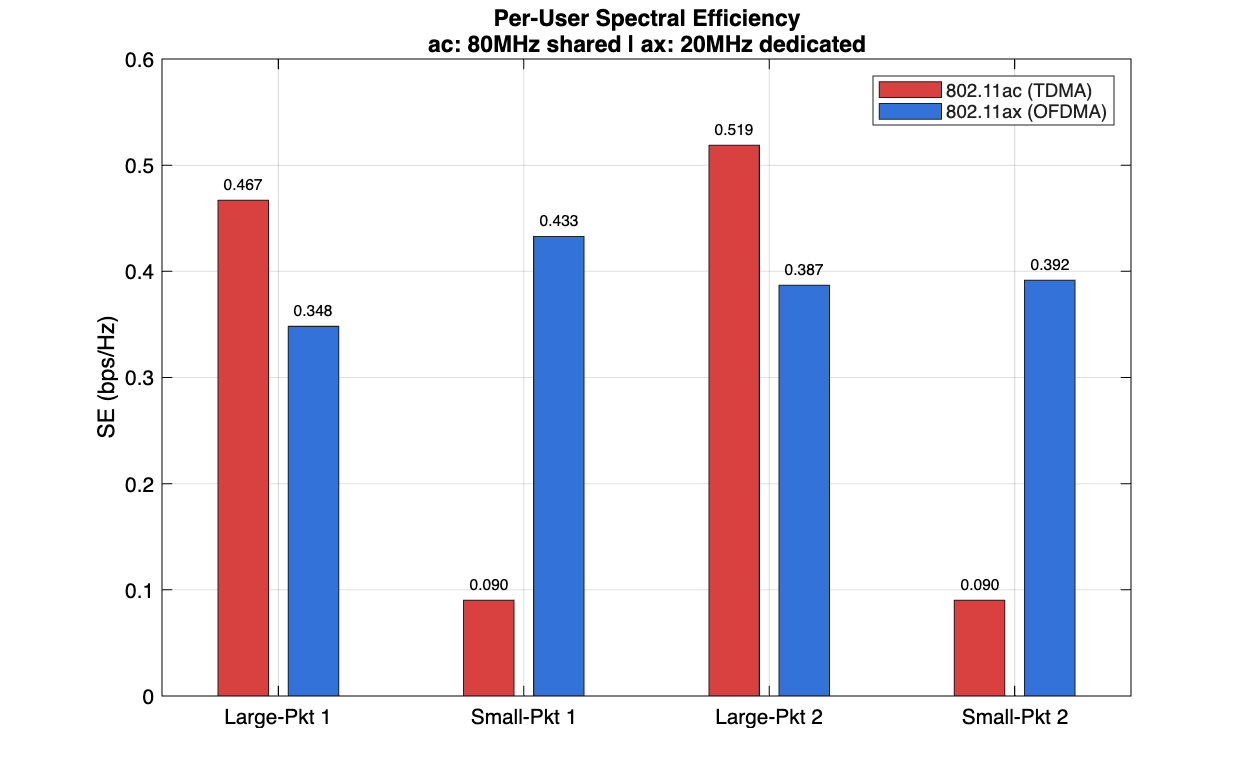
\includegraphics[height=3.9cm]{figures/scenario-a/user_spectral_efficiency.png}
        \caption{Scenario A: Per-user SE (ac: 80\,MHz shared; ax: 20\,MHz dedicated). Small-packet users benefit from OFDMA sub-band assignment.}
        \label{fig:a_user_se}
    \end{minipage}\hfill
\end{figure}

\subsubsection{Delay.}
Average network delay is $\approx$150\,$\mu$s for 802.11ac but $\approx$635\,$\mu$s for 802.11ax. Under TDMA, voice users (position~1 or~2 in the round) experience short slot durations with low queuing overhead ($\approx$80--100\,$\mu$s), while video users further down the round accumulate more queuing ($\approx$200\,$\mu$s). Under OFDMA, every user is charged the same bottleneck slot ($\approx$635\,$\mu$s), dominated by the video frames. This is a direct consequence of having heterogeneous frame sizes in a flat OFDMA allocation.

\subsection{Scenario B: Variable SNR (Near vs.\ Far Users)}

\subsubsection{Setup and Hypothesis.}
Four users were placed at 3--9\,m with SNRs of 38, 34, 12, and 8\,dB. Two near users transmitted 1024\,B at MCS~9/11, while two far users used 512\,B at MCS~2/3 and MCS~1/2. We hypothesised that OFDMA should allow far users to receive dedicated RUs without being squeezed out by near users. However, the large SNR spread (up to 30\,dB difference) means the near users' high-MCS, large frames would likely set a long bottleneck slot, and the far users would not be able to compensate with their low MCS within that same slot. OFDMA was therefore not expected to provide a clear fairness or throughput benefit in this scenario.

\subsubsection{Throughput.}
\autoref{fig:b_total_tp} shows 802.11ac achieving 76.7\,Mbps versus only 18.2\,Mbps for 802.11ax — again a $4\times$ gap. The per-user breakdown (\autoref{fig:b_user_tp}) is revealing: near users drop from $\approx$36.5\,Mbps (802.11ac) to 5.6--10.2\,Mbps (OFDMA), while far users drop even more sharply, from 8.1--8.5\,Mbps to only 1.4--1.6\,Mbps. In TDMA, far users receive a dedicated short slot tuned to their small 512\,B payload, which they can use reasonably efficiently. In OFDMA, the shared slot is set by the near users' large 1024\,B frames at MCS~11, effectively giving far users a very long window in which they can transmit very little data at low MCS.

\begin{figure}
    \begin{minipage}{0.45\textwidth}
        \centering
        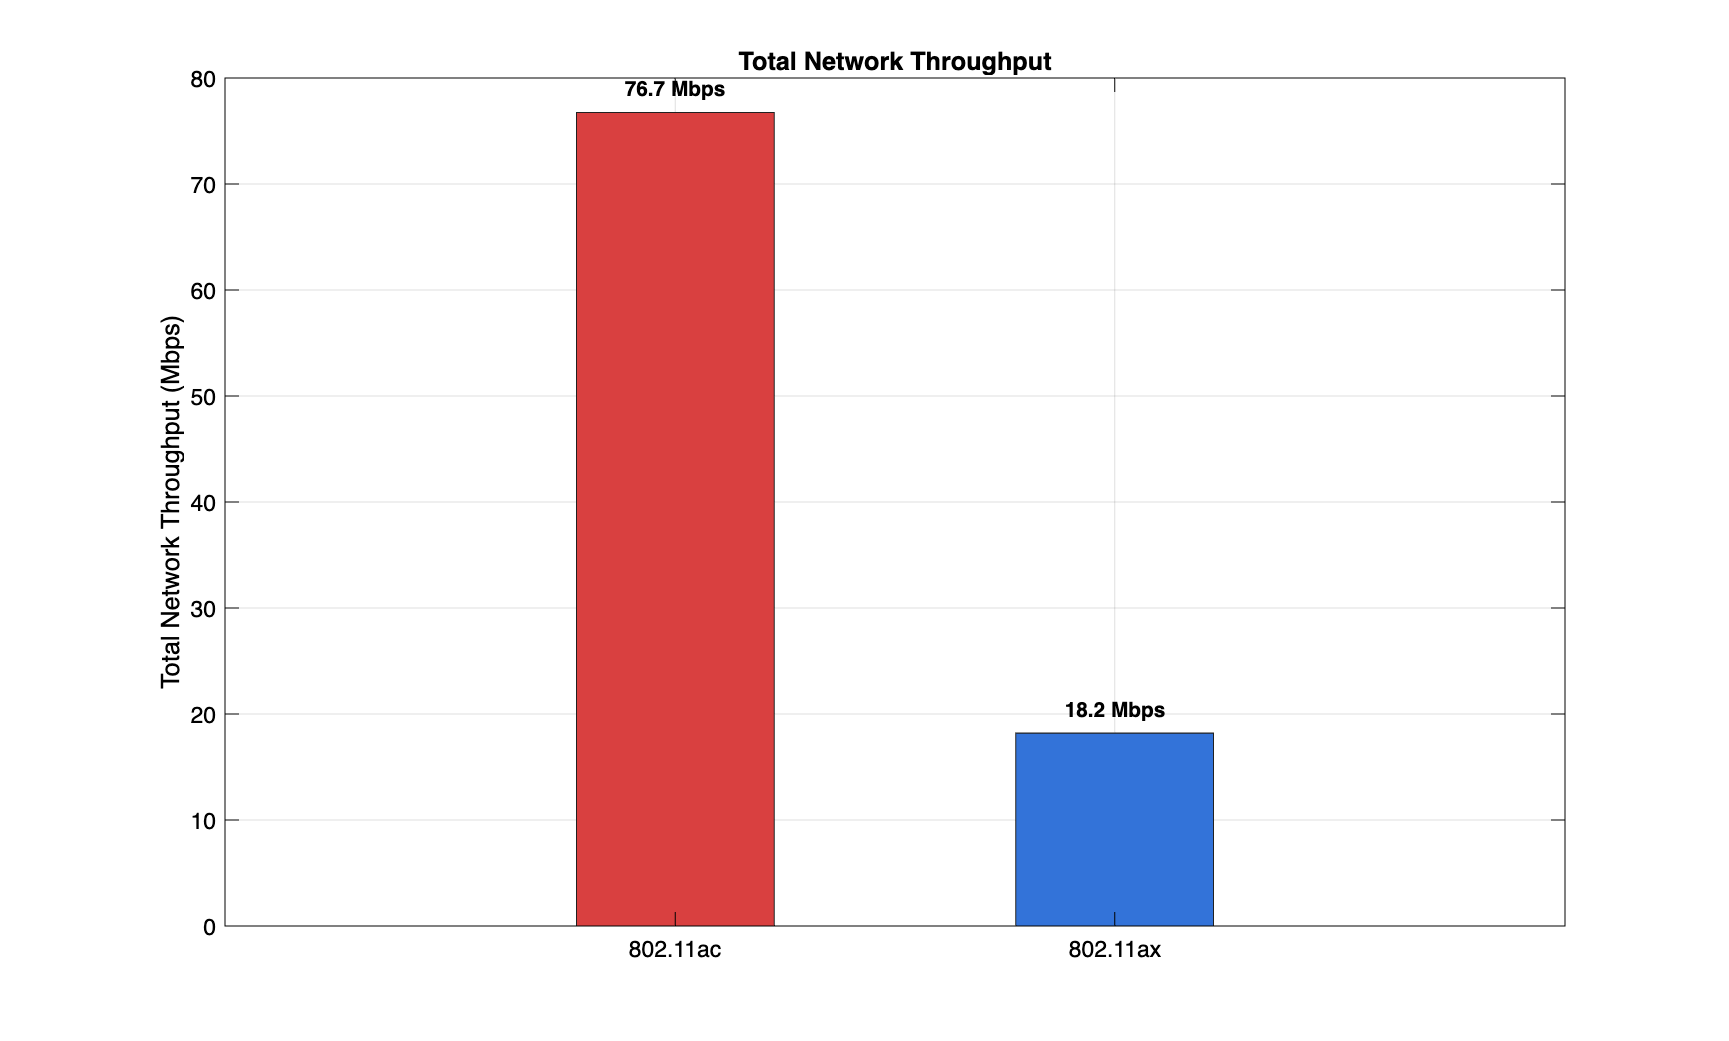
\includegraphics[height=3.9cm]{figures/scenario-b/total_network_throughput.png}
        \caption{Scenario B: Total network throughput. The throughput gap between ac and ax widens under high SNR spread.}
        \label{fig:b_total_tp}
    \end{minipage}\hfill
\end{figure}

\begin{figure}
    \begin{minipage}{0.45\textwidth}
        \centering
        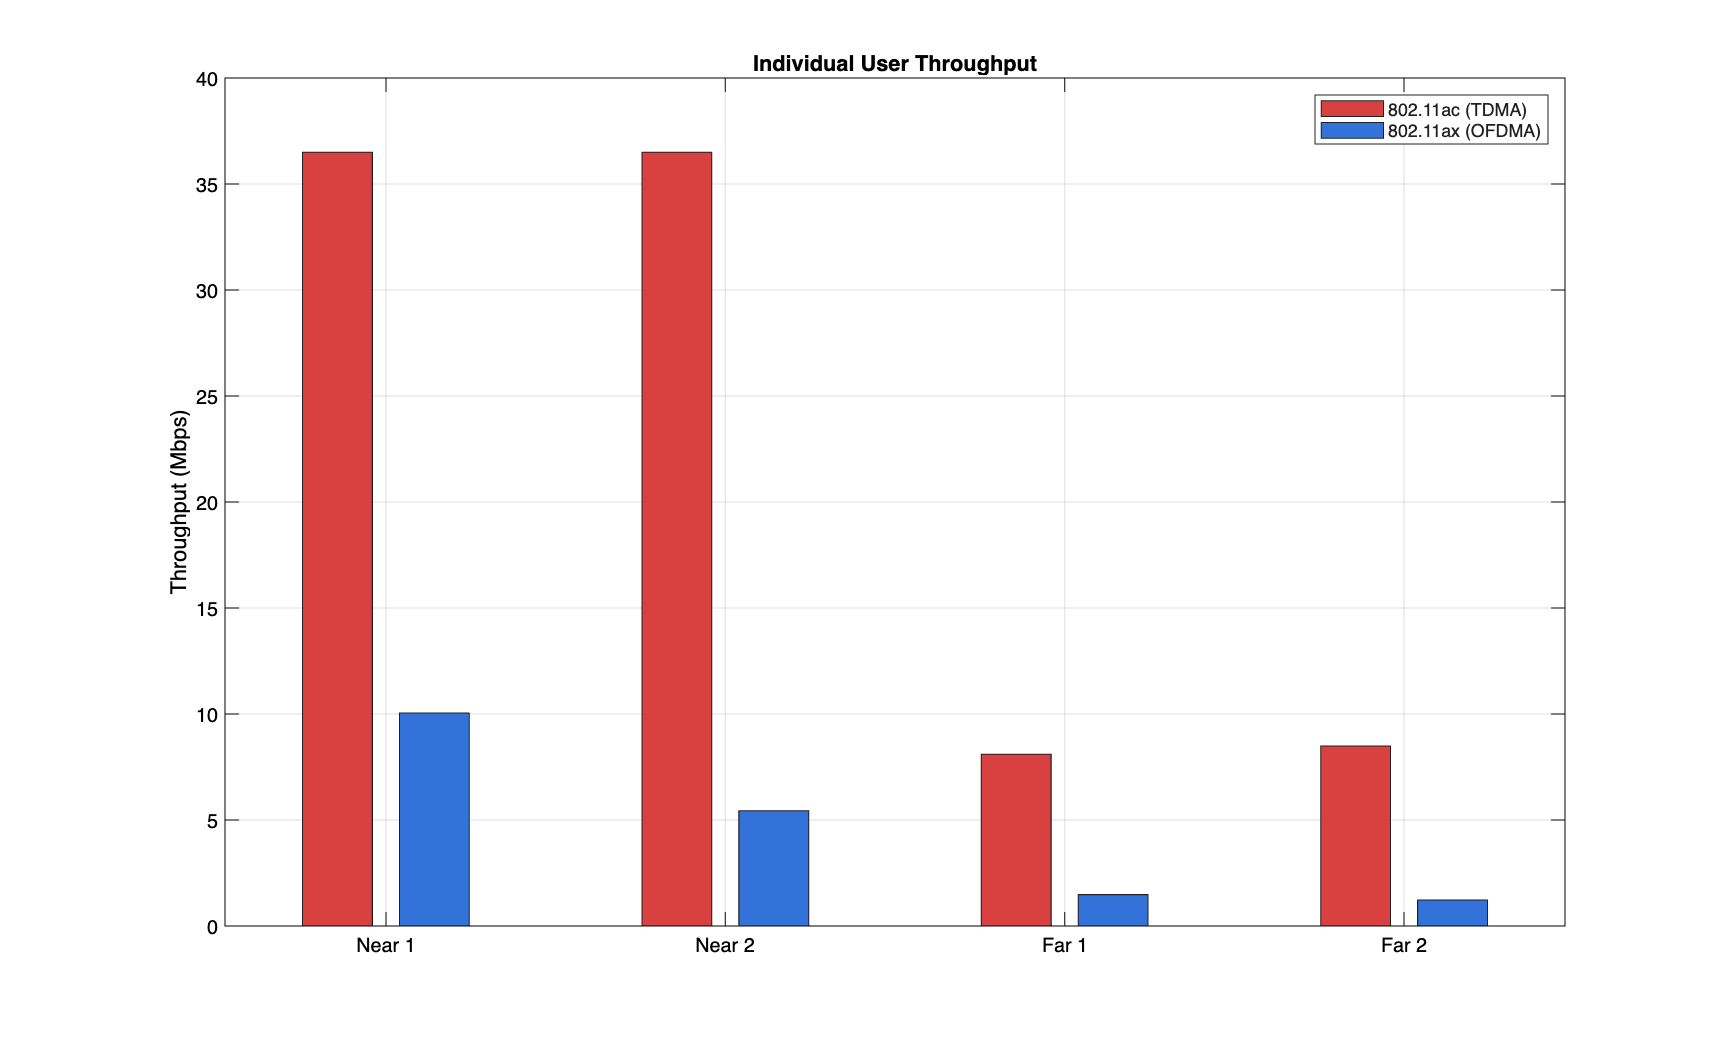
\includegraphics[height=3.9cm]{figures/scenario-b/individual_user_throughput.png}
        \caption{Scenario B: Per-user throughput. Far users suffer most under OFDMA due to MCS mismatch with the bottleneck slot.}
        \label{fig:b_user_tp}
    \end{minipage}\hfill
\end{figure}

\subsubsection{Fairness and Delay.}
The fairness result is counterintuitive: 802.11ax \emph{reduces} Jain's Fairness Index from 0.735 (802.11ac) to 0.620 (\autoref{fig:b_jfi}), the opposite of Scenario A. This is because the near-far SNR spread is so extreme that OFDMA cannot overcome the MCS disparity within a shared slot. Near users extract many more bits per slot than far users, and since the slot duration is set by the near users, far users are disproportionately penalised. Round-robin TDMA, by contrast, gives each user a slot sized to their own frame — a form of implicit per-user adaptation that OFDMA, in its flat allocation, cannot replicate. Average delay also rises dramatically, from $\approx$230\,$\mu$s (802.11ac) to $\approx$1000\,$\mu$s (802.11ax) — a $4\times$ increase driven by the near users' long 1024\,B frames at MCS~11 setting the bottleneck slot for everyone.

\begin{figure}
    \begin{minipage}{0.45\textwidth}
        \centering
        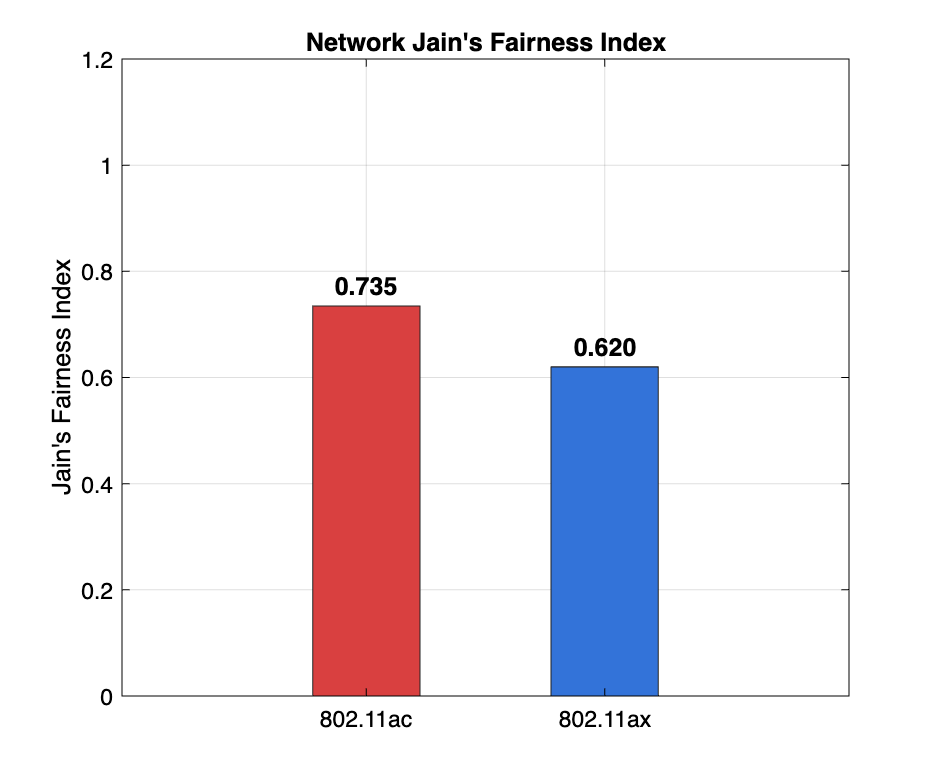
\includegraphics[height=3.9cm]{figures/scenario-b/jain_fairness_index.png}
        \caption{Scenario B: Jain's Fairness Index. Contrary to Scenario A, OFDMA \emph{worsens} fairness when SNR spread is large.}
        \label{fig:b_jfi}
    \end{minipage}\hfill
\end{figure}

\section{Limitations}

The most significant limitation is the use of a single 996-tone RU (allocation index~112) for all users in OFDMA, assigning each user the full 80\,MHz channel in parallel. A practical 802.11ax deployment would subdivide the band into smaller RUs per user (e.g., four 242-tone RUs in 80\,MHz), reducing per-user bandwidth while enabling true frequency reuse. Our model captures the temporal sharing gain of OFDMA (one bottleneck slot instead of $N$ sequential slots) but not the full multiplexing advantage, making the results conservative for OFDMA. In addition, 802.11ax supports padding and RU-size adaptation to align frame durations across users, which would mitigate the bottleneck-slot penalty.

Large-scale fading was disabled, meaning users at their given distances experience only small-scale multipath variations. This likely underestimates SNR variance in real deployments. The simulation also assumes perfect channel knowledge at the receiver, SISO links, and a static round-robin scheduler rather than a channel-aware or QoS-aware one. Finally, 50 packets per user is a small sample, and drop-rate statistics are not fully converged.

\section{Conclusions}

The two simulation scenarios present a nuanced picture of 802.11ax OFDMA versus 802.11ac TDMA. In Scenario A (heterogeneous traffic), OFDMA substantially improves fairness (JFI: $0.675 \to 0.994$) and benefits small-packet users in terms of per-user spectral efficiency, at the cost of lower aggregate throughput and higher average delay. In Scenario B (variable SNR), OFDMA is harmful across all metrics: aggregate throughput is $4\times$ lower, fairness is actually worse ($0.735 \to 0.620$), and delay rises to $\approx$1000\,$\mu$s. The root cause is consistent across both scenarios: the bottleneck-slot effect. When user frames differ greatly in size or in the number of bits they can reliably carry per symbol, binding all users to the same slot duration is wasteful.

These results suggest that OFDMA primarily offers a fairness benefit when user traffic is mixed in payload size but not dramatically different in channel quality. When SNR spread is large, TDMA's implicit per-user frame-size adaptation is actually a form of fairness that OFDMA's flat allocation cannot match. Real 802.11ax deployments address this through fine-grained RU assignment and per-user MCS optimisation, making those scheduling mechanisms the critical enabler of OFDMA gains — an aspect worth exploring in future work.

\section{References}

\begin{thebibliography}{9}

\bibitem{ieee80211ax}
    IEEE Std 802.11ax-2021, \textit{IEEE Standard for Information Technology: Wireless LAN MAC and PHY Specifications — Amendment 1: Enhancements for High-Efficiency WLAN}, IEEE, 2021.

\bibitem{matlab_wlan}
    MathWorks, \textit{WLAN Toolbox User's Guide}, The MathWorks, Inc., 2024. [Online]. Available: \texttt{https://www.mathworks.com/products/wlan.html}

\bibitem{bellalta2016}
    B. Bellalta, ``IEEE 802.11ax: High-efficiency WLANs,'' \textit{IEEE Wireless Communications}, vol.~23, no.~1, pp.~38--46, Feb.~2016.

\bibitem{khorov2019}
    E. Khorov, A. Kiryanov, A. Lyakhov, and G. Bianchi, ``A tutorial on IEEE 802.11ax high efficiency WLANs,'' \textit{IEEE Communications Surveys \& Tutorials}, vol.~21, no.~1, pp.~197--216, 2019.

\end{thebibliography}

\end{document}
